\chapter{シミュレーションによる評価} \label{chapter:evaluate}
本章では、提案した手法の評価を行う。
\ref{section:評価方法}節では、評価方法について述べる。
\ref{section:実験条件}節では、シミュレーション実験の条件について述べる。
\ref{section:結果}節では、シミュレーション実験の結果を述べる。
\ref{section:考察}節では、考察について述べる。

%%%%%%%%%%%%%%%%%%%%%%%%%%%%%%%%%%%%%%%%%%%%%%%%%%%%%%%%%%%%%%%%%%%%%%%%%%%%%%%%
\section{評価方法} \label{section:評価方法}
本節では、評価方法について述べる。
まず、評価を行うにあたって、本手法により目指している動作について述べる。
そして、その目指している動作を達成しているかを評価するときの基準について述べる。

%%%%%%%%%%%%%%%%%%%%%%%%%%%%%%%%%%%%%%%%
\subsection{目指している動作}
本論文において、移動ロボットに行わせたい動作は、状態推定の不確かさを考慮した障害物回避の動作である。
通常行われるような、最も確率の高い姿勢を真の姿勢と仮定して行われる行動計画では、確率的な推定の情報が行動に生かされない。
そこで、信念分布内のどこかにロボットが存在する可能性を考慮し、
信念分布を近似するパーティクル全体が、障害物内に入らないような行動を行わせることを目指している。

また、PFC法のゴール探索動作が行われることも求められる。
分布全体を徐々にゴールになぞるように流し込み、分布内に存在するロボットがいずれゴールへと到達する。
これにより、信念分布がゴール範囲よりも大きい場合でも、ロボットがゴールすることを可能にする。

信念分布が大きい場合この2つの動作を、それぞれ状況にあわせて行うことを目指す。
周囲に障害物があるときには、分布全体が障害物を避けるな動作を行う。
そして、ゴール周辺では、停滞することなくゴールへと到達するするために、分布をゴールへと流し込む探索動作を行う。

%%%%%%%%%%%%%%%%%%%%%%%%%%%%%%%%%%%%%%%%
\subsection{評価方法}
1回のナビゲーションタスクにおいて、障害物の回避とゴールの探索動作がそれぞれ行えているかを評価する。
タスクは、ロボットがゴールへと到達したときに成功とみなす。
逆に、ロボットが障害物内に侵入した時点で、そのタスクは失敗とする。
ロボットがゴールへ到達するのに300秒以上かかった場合も、同様に失敗とする。

ロボットは初期姿勢の配置と動作モデルは、それぞれノイズを有している。
ロボットの初期姿勢は、正規分布に従うばらつきを有しており、
パーティクルの初期分布も、同様の正規分布に従い配置されるものとする。

また、ロボットの状態推定の不確かさが大きい状況を維持するために、
ロボットが観測により得られる情報が非常に制限されているものとする。
自身の姿勢推定に用いることができる情報は、ゴールしているか否かの情報のみである。
これは、PFC法による行動を行うために必要となる観測情報である。
そのほかの距離センサやランドマークによる観測は行えないものとする。

そのために、ロボットがナビゲーションにおいて、状態推定を考慮した障害物回避とゴールの探索を行えているかを
\begin{itemize}
  \item タスクの成功率
  \item タスク成功時の平均時間
  \item 障害物内を移動したパーティクル数×時間 の平均
\end{itemize}
の3つを評価基準とする。
この基準をもとに、提案手法を、通常のPFC法、Q-MDP法、ロボットの真の姿勢による最適方策、
そしてパーティクルの平均姿勢による最適方策の4つと比較する。
各手法それぞれの試行を100回行うことで評価する。


%%%%%%%%%%%%%%%%%%%%%%%%%%%%%%%%%%%%%%%%%%%%%%%%%%%%%%%%%%%%%%%%%%%%%%%%%%%%%%%%
\section{シミュレーション実験の条件} \label{section:実験条件}
本節では、シミュレーションによる実験の条件について述べる。
まず、評価を行うための環境について述べる。
そして、ロボットの初期姿勢や状態遷移確率、行動の種類について述べ、また、MCLやその他パラメータについて述べる。

%%%%%%%%%%%%%%%%%%%%%%%%%%%%%%%%%%%%%%%%
\subsection{環境}
二次元のシミュレータを用いて、評価を行う。
評価は、図\ref{fig:environment}に示すように、一つの障害物を有する、幅が$10[\si{m}]$の正方形の空間で行う。
灰色で示された領域は、障害物を意味する。
また、環境の中央を原点とする$X-Y$座標系$\Sigma$を定義する。
$X$軸と$Y$軸はそれぞれ環境の縁と並行に設定されている。
\begin{figure}[h]
  \begin{center}
    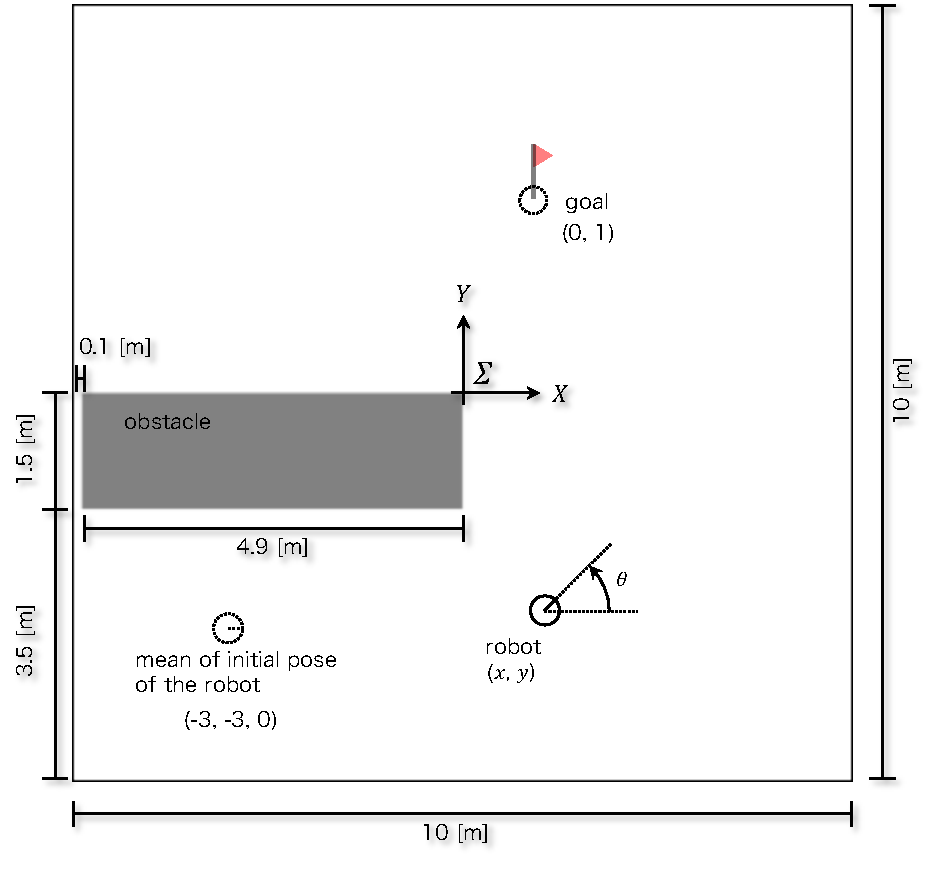
\includegraphics[width=12cm, ]{environment.pdf}
    \caption{Environment map with one obstacle}
    \label{fig:environment}
  \end{center}
\end{figure}

%%%%%%%%%%%%%%%%%%%%%%%%%%%%%%%%%%%%%%%%
\subsection{ロボットの初期姿勢}
ロボットの姿勢$\bm{x}$は、$(x, y, \theta)$で表される。

%%%%%%%%%%%%%%%%%%%%%%%%%%%%%%%%%%%%%%%%
\subsection{MCLの設定}


%%%%%%%%%%%%%%%%%%%%%%%%%%%%%%%%%%%%%%%%%%%%%%%%%%%%%%%%%%%%%%%%%%%%%%%%%%%%%%%%
\section{結果} \label{section:結果}


%%%%%%%%%%%%%%%%%%%%%%%%%%%%%%%%%%%%%%%%%%%%%%%%%%%%%%%%%%%%%%%%%%%%%%%%%%%%%%%%
\section{考察} \label{section:考察}
